

\noindent 
\textbf{\stepcounter{zadatak}
\thecjelina.\thezadatak.}
Dva bloka mase $m_A = 10\ kg$ i $m_B = 8\ kg$ spojena su nerastezljivim užetom i položena na kosinu
nagiba $\alpha = 33^\circ$ kao na slici. Ako je koeficijent kineti\v{c}kog trenja izme\dj{}u bloka A i kosine je 
$\mu_{kA} = 0,4$,
a između bloka B i kosine je $\mu_{kB} = 0,2$ izra\v{c}unajte iznos ubrzanja cijelog sustava.
\begin{figure}[h]%{r}{0.35\textwidth} % Inline image example
  \begin{center}
    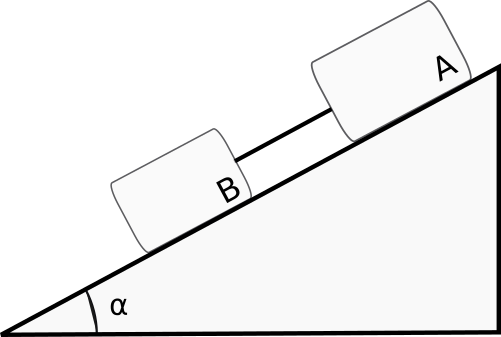
\includegraphics[width=0.3\textwidth]{03_Dinamika_materijalne_tocke/kosina2.png}
  \end{center}
  %\caption{Fish}
\end{figure}

